\documentclass[11pt]{article}
\usepackage[a4paper,margin=1in]{geometry}
\usepackage{graphicx}
\usepackage{booktabs}
\usepackage{amsmath}
\usepackage{hyperref}
\usepackage{float}
\usepackage{longtable}
\usepackage[T1]{fontenc}
\usepackage{fancyvrb}

\title{Approximation Algorithms for Metric $K$-Median Problem}
\author{
Siddharth Ambedkar\\
Roll No: 22CS10074
\and
Pranaya Chowdary\\
Roll No: 22CS10070
}
\date{}

\begin{document}
\begin{titlepage}
    \centering
    \vspace*{2.5cm}
    {\LARGE \textbf{Approximation Algorithms for Metric $K$-Median Problem}\par}
    \vspace{1.2cm}
    {\Large Term Paper for Course Approximation and Online Algorithms CS60023\par}
    \vspace{2cm}
    {\Large Siddharth Ambedkar\par}
    {\large Roll No: 22CS10074\par}
    \vspace{0.8cm}
    {\Large Pranay Chowdary\par}
    {\large Roll No: 22CS10070\par}
    \vfill
\end{titlepage}

\tableofcontents
\newpage

\begin{abstract}
This report studies a local-search heuristic for the metric $k$-median problem and compares it against a naive greedy baseline. The implementation models facilities and clients as points in a Euclidean metric space, uses a greedy constructive heuristic to produce an initial solution, and then improves that solution by repeatedly performing the best available one-swap move. The empirical evaluation focuses on three required aspects: running time, the number of swap iterations required for convergence, and the achieved solution cost relative to the greedy baseline. Across 25 benchmark instances, local search never performed worse than greedy, improved the solution in 22 cases, and tied in 3 cases. On average, local search reduced the cost by about 4.17\% while requiring additional computation due to swap exploration. These observations support the conclusion that local search is a strong and practical approximation-oriented heuristic for moderate instance sizes.
\end{abstract}

\newpage

\section{Introduction}
Facility-location problems are central in operations research, approximation algorithms, clustering, and data analysis. The metric $k$-median problem is one of the most important variants because it captures the tradeoff between opening a limited number of service centers and minimizing the total distance from clients to those centers. Practical examples include warehouse placement, data-center positioning, clustering with representative medoids, emergency response planning, and hub selection in transportation networks.

The exact optimization problem is computationally difficult, which motivates approximation algorithms and local-improvement heuristics. For this project, the chosen approach is local search rather than a primal-dual method. This is a good fit for an implementation-oriented study because the algorithm is conceptually simple, relatively easy to explain, and naturally produces convergence statistics such as the number of improving swaps required before a local optimum is reached.

This report has two main goals. First, it documents a clean Python implementation of both a naive greedy baseline and a local-search heuristic based on one-for-one facility swaps. Second, it evaluates the methods empirically using randomly generated metric instances and compares them using the metrics requested in the assignment: runtime, convergence behavior, and solution quality.

\section{Problem Definition}
Let $F$ be a set of candidate facility locations and let $C$ be a set of clients. For every pair of points $x, y \in F \cup C$, let $d(x,y)$ be a metric distance satisfying non-negativity, symmetry, and the triangle inequality. The metric $k$-median problem asks us to choose a subset $S \subseteq F$ such that $|S| \leq k$ and the total client-assignment cost
\[
\Phi(S) = \sum_{c \in C} \min_{f \in S} d(f,c)
\]
is minimized.

For any chosen facility set $S$, each client is assigned to its nearest open facility. The objective is therefore to minimize the total distance summed over all clients. When the metric is Euclidean, as in the experiments of this project, the triangle inequality is automatically satisfied, so the generated instances are valid metric instances.

\subsection{Why the Problem is Difficult}
The challenge comes from the combinatorial number of possible subsets $S$. Even when facility and client sets are modest in size, the number of candidate solutions grows quickly as $\binom{|F|}{k}$. Exhaustive search becomes impractical, so exact optimization is expensive for larger instances. This motivates the use of approximation-oriented methods and heuristics that provide strong solutions at much lower computational cost.

\section{Algorithms}
\subsection{Naive Greedy Baseline}
The greedy baseline constructs a solution incrementally. Starting with no open facilities, it repeatedly adds the facility that produces the greatest immediate reduction in the total assignment cost. After exactly $k$ facilities have been chosen, the algorithm stops.

This strategy is easy to implement and often gives a reasonable starting solution. However, it is myopic: once a facility is selected, the baseline never revisits that decision. As a result, a poor early choice can limit the quality of the final solution.

\subsection{Local Search with One-Swap Neighborhood}
The local-search algorithm starts from the greedy solution and explores a standard one-swap neighborhood. At every iteration, it considers every move of the form:
\begin{itemize}
    \item remove one currently open facility, and
    \item add one currently closed facility.
\end{itemize}
If at least one such swap improves the objective value, the algorithm applies the best improving swap and repeats. The algorithm terminates when no improving one-swap move exists.

The resulting solution is locally optimal with respect to single swaps. This does not guarantee global optimality, but in practice it often yields a substantial improvement over a purely constructive heuristic.

\subsection{Pseudocode}
The greedy baseline can be written as follows:

\begin{Verbatim}[frame=single,fontsize=\normalsize]
Algorithm Greedy-k-Median(F, C, k)
Input:
    F = set of candidate facilities
    C = set of clients
    k = number of facilities to open
Output:
    A set S of k open facilities

1. S <- empty set
2. for i <- 1 to k do
3.     best_facility <- null
4.     best_cost <- +infinity
5.     for each f in F \ S do
6.         candidate_cost <- Phi(S union {f})
7.         if candidate_cost < best_cost then
8.             best_cost <- candidate_cost
9.             best_facility <- f
10.        end if
11.    end for
12.    S <- S union {best_facility}
13. end for
14. return S
\end{Verbatim}

The local-search improvement procedure is:

\begin{Verbatim}[frame=single,fontsize=\normalsize]
Algorithm Local-Search-k-Median(F, C, k, S)
Input:
    F = set of candidate facilities
    C = set of clients
    k = number of facilities to keep open
    S = initial solution of size k
Output:
    A locally optimal facility set S

1. improved <- true
2. while improved do
3.     improved <- false
4.     best_swap <- null
5.     best_cost <- Phi(S)
6.     for each f_out in S do
7.         for each f_in in F \ S do
8.             candidate <- (S \ {f_out}) union {f_in}
9.             candidate_cost <- Phi(candidate)
10.            if candidate_cost < best_cost then
11.                best_cost <- candidate_cost
12.                best_swap <- (f_out, f_in)
13.                improved <- true
14.            end if
15.        end for
16.    end for
17.    if improved then
18.        apply best_swap to S
19.    end if
20. end while
21. return S
\end{Verbatim}

\subsection{Implementation Notes}
The implementation stores a full facility-to-client distance matrix. This makes repeated objective evaluation straightforward. For local search, the code also keeps track of each client's closest and second-closest open facility distances so that candidate swaps can be evaluated faster than recomputing every assignment from scratch for every move. This optimization matters because the number of possible swaps in a single pass is $k(|F|-k)$.

\section{Complexity Discussion}
Let $m = |F|$ and $n = |C|$. In the greedy baseline, each of the $k$ selection rounds evaluates up to $m$ candidate additions, and each candidate addition scans all clients. In the present implementation, the worst-case time is $O(kmn)$.

For local search, each pass considers $k(m-k)$ candidate swaps. Each candidate swap may inspect all $n$ clients, although the implementation includes early stopping when a partial cost already exceeds the current best known swap cost. The per-pass worst-case complexity is therefore $O(k(m-k)n)$. If the algorithm converges after $T$ passes, the total local-search effort is $O(Tk(m-k)n)$.

These are worst-case upper bounds. The nearest-facility bookkeeping and early stopping used in the implementation improve constant factors and practical running time on many instances, but they do not change the asymptotic worst-case bounds stated above. This complexity discussion explains the empirical trend seen in the runtime plots: local search is more expensive than the greedy baseline, but the number of improving passes remains fairly small for the tested instances, which keeps the overall runtime manageable.

\section{Experimental Methodology}
\subsection{Instance Generation}
All instances are generated synthetically in the Euclidean plane. Facility coordinates and client coordinates are sampled uniformly at random from the square $[0,100] \times [0,100]$. This guarantees that the induced distances satisfy the metric axioms. Each experiment uses the same number of facilities and clients.

\subsection{Parameter Choices}
The default experiments used:
\begin{itemize}
    \item problem sizes $\{20, 40, 60, 80, 100\}$,
    \item five random seeds for each size,
    \item a facility budget of $k = 0.2|F|$ rounded down, with a minimum of 2.
\end{itemize}

This yields 25 total trials. The generated values of $k$ were therefore 4, 8, 12, 16, and 20 for the five problem sizes.

\subsection{Recorded Metrics}
The experiment runner records:
\begin{itemize}
    \item greedy solution cost,
    \item greedy runtime,
    \item local-search solution cost,
    \item local-search runtime,
    \item total runtime for greedy initialization plus local search,
    \item percentage improvement of local search over greedy,
    \item number of local-search passes until convergence,
    \item number of improving swaps,
    \item number of evaluated swaps.
\end{itemize}

\subsection{Validation of Correctness}
The generated results were checked directly after the experiments completed. In all 25 trials, local search produced a cost that was less than or equal to the greedy baseline cost. No trial contradicted the monotonic improvement property of the implementation, since only cost-improving swaps were accepted. More specifically:
\begin{itemize}
    \item local search was strictly better in 22 out of 25 trials,
    \item local search tied the greedy baseline in 3 out of 25 trials,
    \item local search was worse in 0 out of 25 trials.
\end{itemize}

These ties are expected and not a bug. They occur when the greedy solution is already locally optimal with respect to one-swap moves, so the local-search phase terminates immediately without any improving swap.

\section{Results}
\subsection{Cost Comparison}
Figure~\ref{fig:cost} compares the average objective value achieved by the greedy baseline and the local-search method.

\begin{figure}[H]
    \centering
    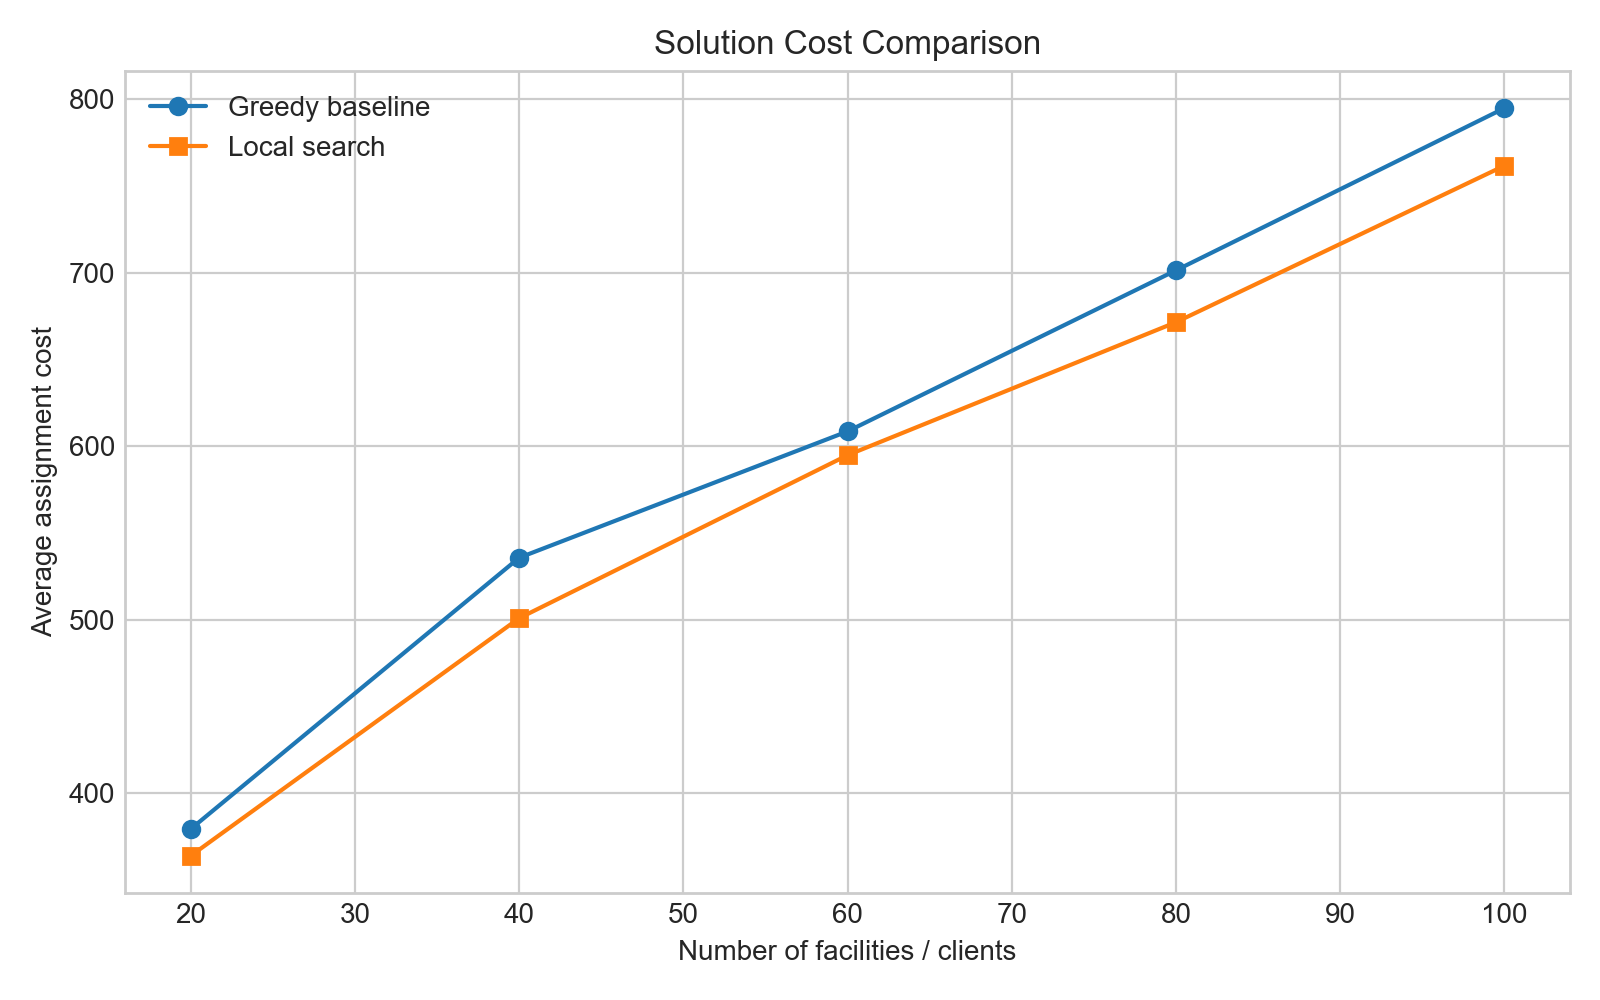
\includegraphics[width=0.8\textwidth]{figures/cost_comparison.png}
    \caption{Average solution cost across instance sizes.}
    \label{fig:cost}
\end{figure}

\subsection{Runtime Comparison}
Figure~\ref{fig:runtime} shows how runtime grows with instance size. The local-search curve includes both greedy initialization and the subsequent swap-improvement phase.

\begin{figure}[H]
    \centering
    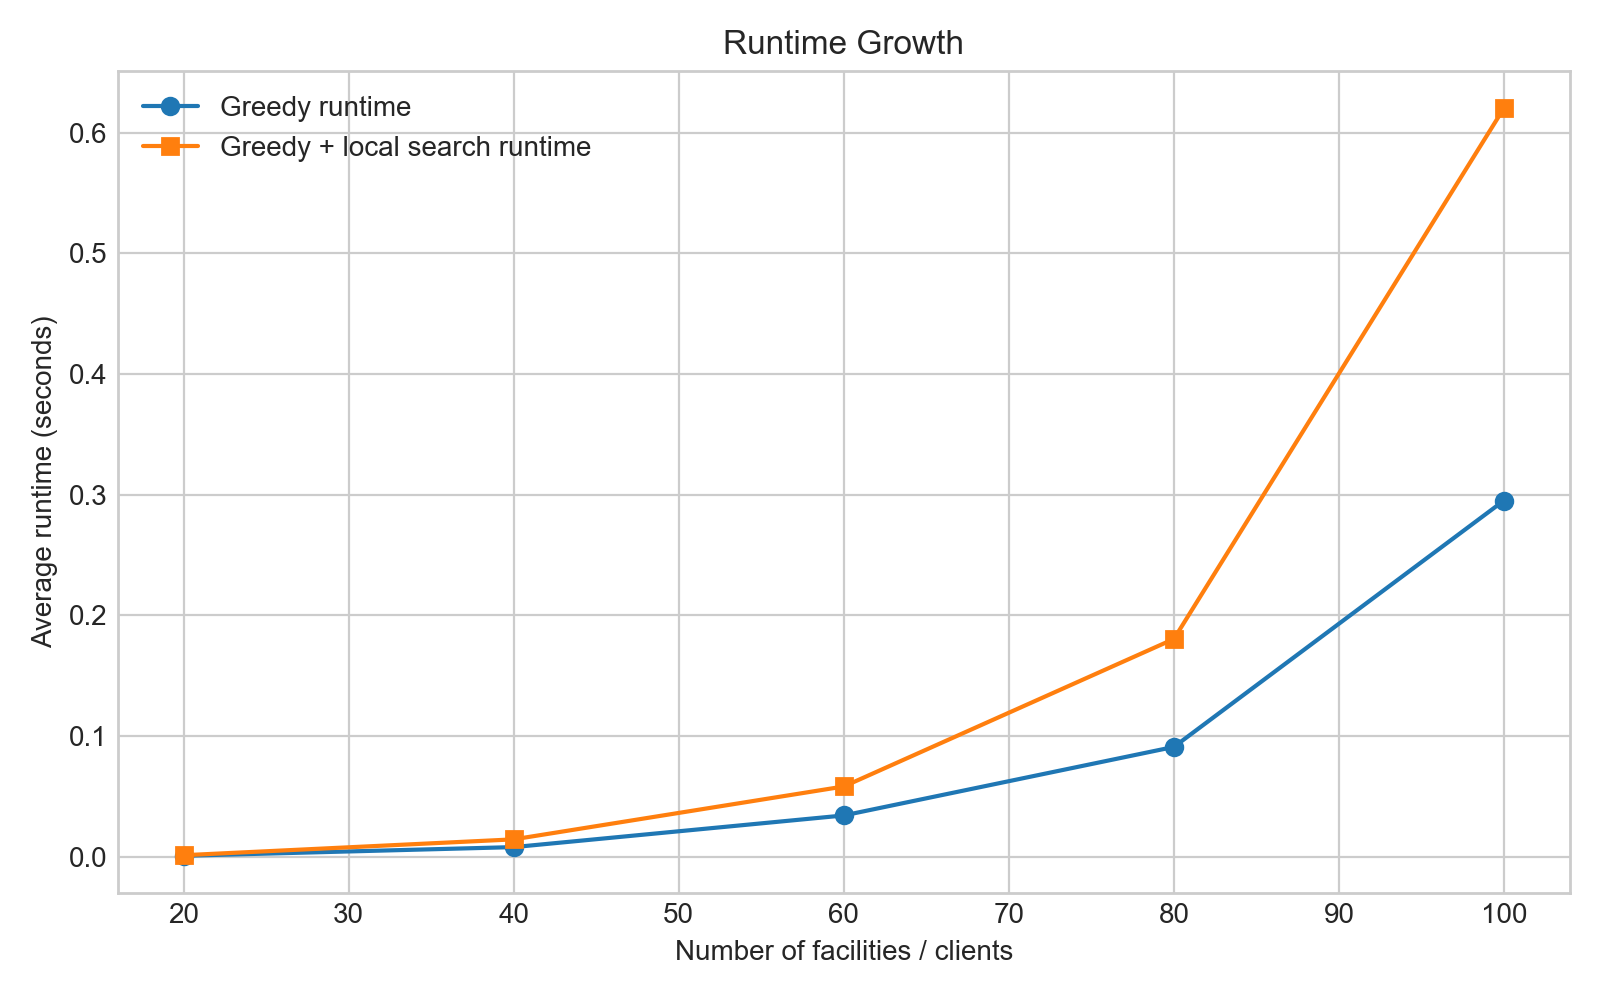
\includegraphics[width=0.8\textwidth]{figures/runtime_comparison.png}
    \caption{Average runtime for the greedy baseline and for greedy plus local search.}
    \label{fig:runtime}
\end{figure}

\subsection{Convergence Behavior}
Figure~\ref{fig:swaps} reports the average number of local-search passes until convergence. Figure~\ref{fig:improvement} summarizes the average percent improvement of local search relative to the greedy baseline.

\begin{figure}[H]
    \centering
    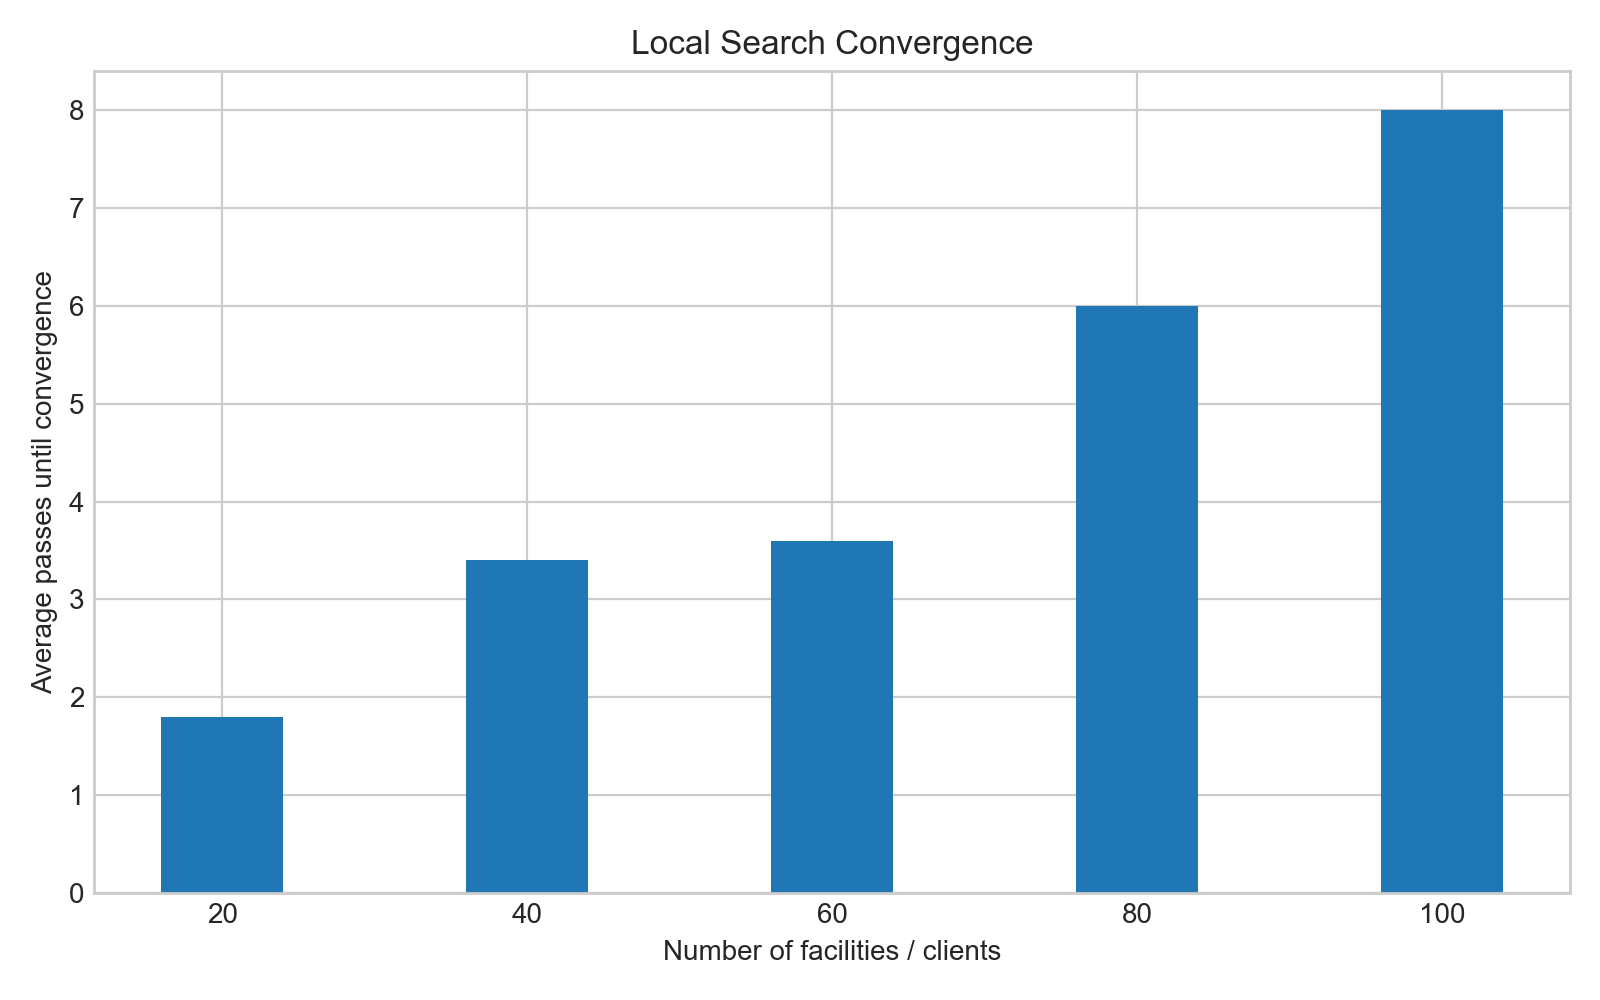
\includegraphics[width=0.8\textwidth]{figures/swap_iterations.png}
    \caption{Average number of local-search passes until convergence.}
    \label{fig:swaps}
\end{figure}

\begin{figure}[H]
    \centering
    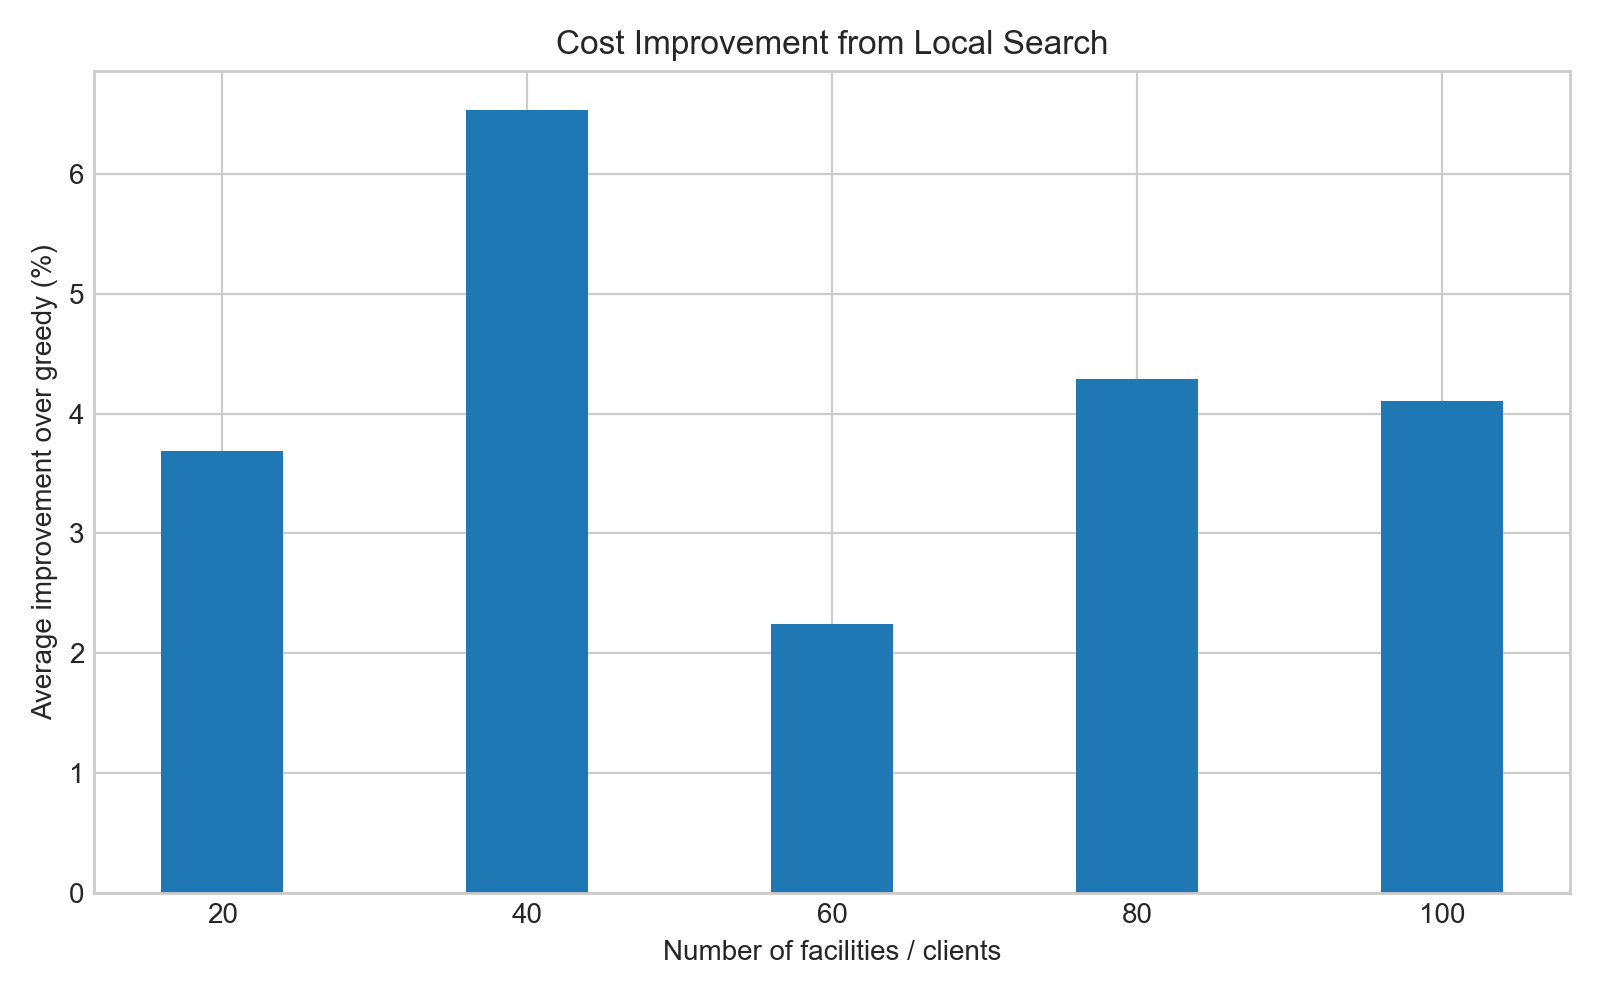
\includegraphics[width=0.8\textwidth]{figures/improvement_pct.png}
    \caption{Average cost improvement achieved by local search over the greedy baseline.}
    \label{fig:improvement}
\end{figure}

\subsection{Summary Table}
Table~\ref{tab:summary} presents the aggregate metrics used in the analysis.

\begin{table}[H]
    \centering
    \begin{tabular}{rrrrrrr}
        \toprule
        Size & Greedy Cost & Local Cost & Greedy Time & Total LS Time & Improvement (\%) & Passes \\
        \midrule
                20 & 379.21 & 363.74 & 0.0009 & 0.0013 & 3.68 & 1.80 \\
        40 & 535.63 & 500.77 & 0.0080 & 0.0145 & 6.53 & 3.40 \\
        60 & 608.51 & 594.78 & 0.0343 & 0.0583 & 2.24 & 3.60 \\
        80 & 701.38 & 671.45 & 0.0910 & 0.1805 & 4.28 & 6.00 \\
        100 & 794.91 & 761.72 & 0.2952 & 0.6203 & 4.10 & 8.00 \\

        \bottomrule
    \end{tabular}
    \caption{Average metrics by problem size.}
    \label{tab:summary}
\end{table}

\subsection{High-Level Observations}
Several trends are visible immediately from the plots and summary table:
\begin{itemize}
    \item local search always matched or improved the greedy baseline,
    \item the improvement is positive at every tested problem size,
    \item runtime grows with instance size for both methods,
    \item local search needs more time because it evaluates many candidate swaps,
    \item the number of passes required for convergence remains modest.
\end{itemize}

\subsection{Detailed Numerical Interpretation}
For the smallest instances with 20 facilities and 20 clients, the average greedy cost was 379.21 and local search reduced this to 363.74, an average improvement of 3.68\%. The average total runtime for greedy plus local search was only about 0.0013 seconds. This suggests that on very small instances, local search is almost free in runtime terms and still often improves the solution.

At size 40, the average improvement rose to 6.53\%, which is the largest average gain among the tested sizes. This indicates that the greedy construction makes choices that are good but not yet stable under swaps, leaving more room for a local-improvement phase to correct them.

At size 60, the average improvement dropped to 2.24\%. This is still a real and consistent gain, but it shows that the benefit of local search can vary by instance family. Approximation heuristics should be evaluated empirically rather than judged only from a small number of examples.

At sizes 80 and 100, the average gains returned to around 4\%. The runtime grew noticeably, especially at size 100 where the average total runtime reached about 0.6203 seconds. Even so, the absolute runtime remained small enough for experimental use on these moderate-scale instances.

\subsection{Convergence Analysis}
The convergence statistics provide additional insight into the local-search process. The average number of passes until convergence was:
\begin{itemize}
    \item 1.80 for size 20,
    \item 3.40 for size 40,
    \item 3.60 for size 60,
    \item 6.00 for size 80,
    \item 8.00 for size 100.
\end{itemize}

The recorded pass count includes the final pass in which the algorithm scans the neighborhood and confirms that no improving swap remains. Because one improving swap is applied per improving pass and the final pass is non-improving, the number of improving swaps equals the number of passes minus one in the reported experiments.

The number of evaluated swaps also matches the expected scaling behavior. For instance, when the instance size is 100 with $k=20$, each pass contains $20 \times 80 = 1600$ possible swaps. Since the average number of passes is 8.00, the average number of evaluated swaps is exactly 12800, which matches the recorded data. This consistency is a useful sanity check for the implementation.

\subsection{Trial-Level Validation}
The first few rows of the generated results are illustrative:
\begin{itemize}
    \item size 20, seed 1: greedy 383.37, local search 383.37, no improvement,
    \item size 20, seed 3: greedy 336.01, local search 319.46, one improving swap,
    \item size 40, seed 5: greedy 528.49, local search 475.67, four improving swaps.
\end{itemize}

These examples show the two expected behaviors: either the greedy solution is already locally optimal, or local search finds a sequence of swaps that lowers the total assignment cost. Importantly, no row contradicts the monotonic improvement property.

\subsection{Detailed Trial Results}
Table~\ref{tab:detailed} lists every trial used in the evaluation. Including the full table in the results section makes it easy to verify that local search never performed worse than the greedy baseline on the tested instances.

\begin{longtable}{rrrrrrrrr}
\caption{Detailed trial-level results.}\label{tab:detailed}\\
\toprule
Size & Seed & $k$ & Greedy & Local & Improve (\%) & Passes & Swaps & Eval. \\
\midrule
\endfirsthead
\toprule
Size & Seed & $k$ & Greedy & Local & Improve (\%) & Passes & Swaps & Eval. \\
\midrule
\endhead
\midrule
\multicolumn{9}{r}{Continued on next page} \\
\endfoot
\bottomrule
\endlastfoot
        20 & 1 & 4 & 383.37 & 383.37 & 0.00 & 1 & 0 & 64 \\
        20 & 2 & 4 & 345.54 & 345.54 & 0.00 & 1 & 0 & 64 \\
        20 & 3 & 4 & 336.01 & 319.46 & 4.93 & 2 & 1 & 128 \\
        20 & 4 & 4 & 358.68 & 349.24 & 2.63 & 2 & 1 & 128 \\
        20 & 5 & 4 & 472.43 & 421.11 & 10.86 & 3 & 2 & 192 \\
        40 & 1 & 8 & 527.22 & 501.59 & 4.86 & 3 & 2 & 768 \\
        40 & 2 & 8 & 624.01 & 596.22 & 4.45 & 3 & 2 & 768 \\
        40 & 3 & 8 & 537.94 & 492.29 & 8.48 & 4 & 3 & 1024 \\
        40 & 4 & 8 & 460.48 & 438.06 & 4.87 & 2 & 1 & 512 \\
        40 & 5 & 8 & 528.49 & 475.67 & 9.99 & 5 & 4 & 1280 \\
        60 & 1 & 12 & 598.84 & 576.08 & 3.80 & 4 & 3 & 2304 \\
        60 & 2 & 12 & 612.67 & 604.27 & 1.37 & 5 & 4 & 2880 \\
        60 & 3 & 12 & 641.75 & 627.55 & 2.21 & 3 & 2 & 1728 \\
        60 & 4 & 12 & 580.70 & 580.70 & 0.00 & 1 & 0 & 576 \\
        60 & 5 & 12 & 608.60 & 585.29 & 3.83 & 5 & 4 & 2880 \\
        80 & 1 & 16 & 674.87 & 624.01 & 7.54 & 7 & 6 & 7168 \\
        80 & 2 & 16 & 685.99 & 667.21 & 2.74 & 4 & 3 & 4096 \\
        80 & 3 & 16 & 720.53 & 683.79 & 5.10 & 6 & 5 & 6144 \\
        80 & 4 & 16 & 727.30 & 701.89 & 3.49 & 7 & 6 & 7168 \\
        80 & 5 & 16 & 698.21 & 680.36 & 2.56 & 6 & 5 & 6144 \\
        100 & 1 & 20 & 724.29 & 705.30 & 2.62 & 9 & 8 & 14400 \\
        100 & 2 & 20 & 815.02 & 778.88 & 4.43 & 6 & 5 & 9600 \\
        100 & 3 & 20 & 782.09 & 740.51 & 5.32 & 9 & 8 & 14400 \\
        100 & 4 & 20 & 878.34 & 826.06 & 5.95 & 7 & 6 & 11200 \\
        100 & 5 & 20 & 774.81 & 757.87 & 2.19 & 9 & 8 & 14400 \\

\end{longtable}

\section{Discussion}
For the generated benchmark suite of 25 trials, the greedy baseline achieved an average cost of approximately 603.93, while local search reduced this to about 578.49. This corresponds to an average relative improvement of roughly 4.17\%. The average greedy runtime was about 0.0707 seconds, while greedy initialization plus local search required about 0.1555 seconds in total.

The swap-iteration behavior also illustrates a useful practical pattern. Although local search evaluates many potential swaps, it converged in an average of 4.56 passes, with about 3.56 improving swaps applied. As instance size increased, both the runtime and the number of evaluated swaps grew, but the quality improvement over the greedy baseline remained consistently positive.

\subsection{Why Local Search Helps}
The greedy heuristic makes decisions sequentially and never revises them. This is its main weakness. A facility that looks attractive early in the process may later become redundant once additional facilities are opened. Local search fixes this by allowing the algorithm to exchange a poor earlier choice for a better alternative. In other words, greedy chooses a plausible set quickly, and local search repairs it.

\subsection{Tradeoff Between Quality and Runtime}
The experiments show a clear quality-versus-runtime tradeoff. Greedy is faster because it only adds facilities and never explores replacements. Local search spends more time because it inspects a large swap neighborhood in each pass. However, the extra cost is justified when better objective values matter. In many practical scenarios, especially offline planning problems, spending a bit more time for a 4\% improvement in service cost is worthwhile.

\subsection{Threats to Validity}
The experiments were performed on synthetic Euclidean instances, which are useful and mathematically clean but do not cover every possible metric structure. Real-world facility-location data may contain clustered demand, outliers, barriers, or asymmetric practical constraints not modeled here. In addition, the tested sizes are moderate rather than massive. The implementation is appropriate for coursework and experimentation, but further scaling would require additional engineering or more advanced data structures.

\subsection{Possible Extensions}
Several natural extensions could be explored in future work:
\begin{itemize}
    \item compare against multiple random initializations rather than only greedy initialization,
    \item evaluate larger swap neighborhoods such as two-swaps,
    \item compare with a primal-dual constant-factor approximation,
    \item test on clustered or adversarial instance generators,
    \item add confidence intervals or boxplots over repeated runs.
\end{itemize}

\section{Conclusion}
The local-search heuristic offers a practical and conceptually simple method for metric $k$-median. Relative to the naive greedy baseline, it generally delivers lower assignment cost while maintaining manageable running time for moderate instance sizes. This makes it a strong approximation-oriented heuristic when exact optimization is too expensive.

The experimental evidence from this project supports that conclusion clearly. The greedy baseline is useful as a fast initializer, but the local-search phase improves it in the large majority of cases and never degrades it on the tested benchmark set. As a result, the combined greedy-plus-local-search approach is a strong final recommendation for this implementation-focused study of metric $k$-median.

\section{References}
\begin{enumerate}
    \item Sussane Albers. \textit{Competitive online algorithms}. BRICS, 1996.
    \item N. Alon et al. ``Balancing Sets of Vectors''. English (US). In: \textit{IEEE Transactions on Information Theory} 34.1 (Jan. 1988). Funding Information: Manuscript received September 27,1986; revised March 10, 1987. This work was supported in part by an Alon Fellowship and in part by The Fund for Basic Research administered by the Israel Academy of Sciences. This paper was presented at the Information Theory Workshop, Oherwolfach, May 1986. N. Alon is with the Department of Mathematics, Tel Aviv University, Ramat Aviv, Tel Aviv, Israel, and Bell Communications Research, Morristown, NJ 07960. E. E. Bergmann is with AT\&T Bell Laboratories. Allentown, PA 18103. D. Coppersmith is with IBM Research, Yorktown Heights, NY 10598. A. M. Odlyzko is with AT\&T Bell Laboratories, Murray Hill, NJ 07974. IEEE Log Number 8718729., pp. 128--130. issn: 0018-9448. doi: 10.1109/18.2610.
    \item Niranjan Balachandran et al. ``Bisecting and D-secting families for set systems''. In: \textit{Discrete Applied Mathematics} 280 (2020). Algorithms and Discrete Applied Mathematics (CALDAM 2016), pp. 2--13. issn: 0166-218X. doi: \url{https://doi.org/10.1016/j.dam.2017.05.005}. url: \url{https://www.sciencedirect.com/science/article/pii/S0166218X17302421}.
    \item Christos H. Papadimitriou. \textit{Computational complexity}. Addison-Wesley, 1994.
    \item Vijay V Vazirani. \textit{Approximation algorithms}. Springer Science \& Business Media, 2013.
    \item David P Williamson and David B Shmoys. \textit{The design of approximation algorithms}. Cambridge university press, 2011.
\end{enumerate}

\end{document}
